\documentclass[tikz, border=6pt]{standalone}
\usepackage[T1]{fontenc}
\usepackage{lmodern}
\usepackage{amsmath,amssymb,bm}
\usepackage[scaled=0.95]{helvet}
\usetikzlibrary{arrows.meta}
\definecolor{Blue}{HTML}{3A76D8}
\definecolor{Red}{HTML}{DF4B4B}
\definecolor{Ink}{HTML}{1F2937}
\tikzset{
  dot/.style={circle, fill, inner sep=0pt, minimum size=4.5pt},
  block/.style={/utils/exec={\colorlet{pytikzarg}{#1}}, draw=pytikzarg!78!black, fill=pytikzarg!14, rounded corners=3pt, align=center, inner sep=5pt, minimum height=8mm, minimum width=20mm},
  block/.default=Blue,
  op/.style={circle, draw, fill=white, inner sep=0pt, minimum size=5mm, font=\normalsize},
}
\begin{document}
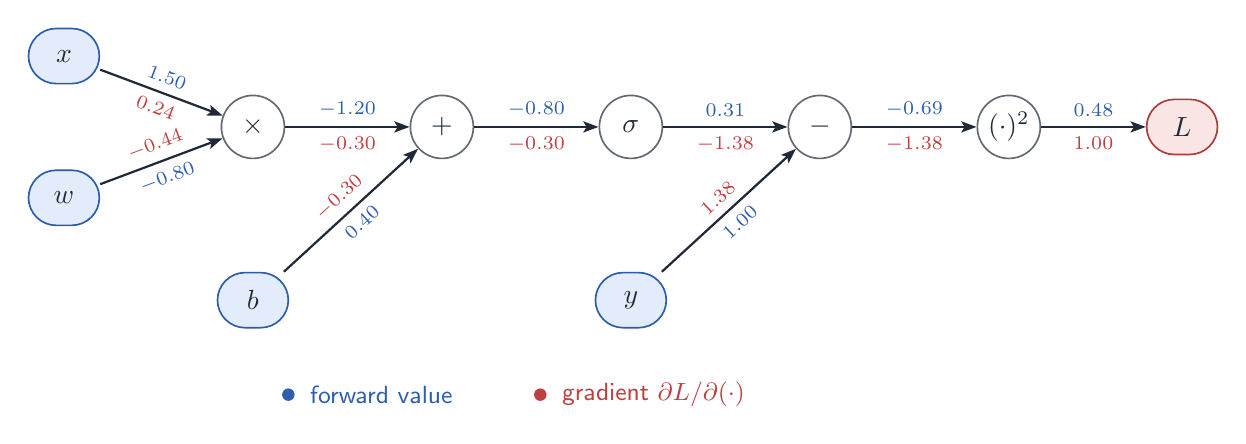
\begin{tikzpicture}[color=Ink, execute at begin picture={\sffamily}, line width=0.6pt, >={Stealth[length=5.5pt, width=4pt, inset=1.2pt]}, line join=round]
  \node[block=Blue, minimum width=0.9cm, minimum height=0.7cm, rounded corners=10pt] (n1) at (0,1.2) {$x$};
  \node[block=Blue, minimum width=0.9cm, minimum height=0.7cm, rounded corners=10pt] (n2) at (0,-0.6) {$w$};
  \node[block=Blue, minimum width=0.9cm, minimum height=0.7cm, rounded corners=10pt] (n3) at (2.4,-1.9) {$b$};
  \node[block=Blue, minimum width=0.9cm, minimum height=0.7cm, rounded corners=10pt] (n4) at (7.2,-1.9) {$y$};
  \node[op, minimum size=0.8cm, draw=Ink!70] (n5) at (2.4,0.3) {$\times$};
  \node[op, minimum size=0.8cm, draw=Ink!70] (n6) at (4.8,0.3) {$+$};
  \node[op, minimum size=0.8cm, draw=Ink!70] (n7) at (7.2,0.3) {$\sigma$};
  \node[op, minimum size=0.8cm, draw=Ink!70] (n8) at (9.6,0.3) {$-$};
  \node[op, minimum size=0.8cm, draw=Ink!70] (n9) at (12,0.3) {$(\cdot)^2$};
  \node[block=Red, minimum width=0.9cm, minimum height=0.7cm, rounded corners=10pt] (n10) at (14.2,0.3) {$L$};
  \draw[->, line width=0.8pt] (n1) -- (n5);
  \path (n1) -- node[above, sloped, font=\scriptsize, text=Blue!80!black, pos=0.5] {$1.50$} (n5);
  \path (n1) -- node[below, sloped, font=\scriptsize, text=Red!85!black, pos=0.5] {$0.24$} (n5);
  \draw[->, line width=0.8pt] (n2) -- (n5);
  \path (n2) -- node[below, sloped, font=\scriptsize, text=Blue!80!black, pos=0.5] {$-0.80$} (n5);
  \path (n2) -- node[above, sloped, font=\scriptsize, text=Red!85!black, pos=0.5] {$-0.44$} (n5);
  \draw[->, line width=0.8pt] (n5) -- (n6);
  \path (n5) -- node[above, sloped, font=\scriptsize, text=Blue!80!black, pos=0.5] {$-1.20$} (n6);
  \path (n5) -- node[below, sloped, font=\scriptsize, text=Red!85!black, pos=0.5] {$-0.30$} (n6);
  \draw[->, line width=0.8pt] (n3) -- (n6);
  \path (n3) -- node[below, sloped, font=\scriptsize, text=Blue!80!black, pos=0.5] {$0.40$} (n6);
  \path (n3) -- node[above, sloped, font=\scriptsize, text=Red!85!black, pos=0.5] {$-0.30$} (n6);
  \draw[->, line width=0.8pt] (n6) -- (n7);
  \path (n6) -- node[above, sloped, font=\scriptsize, text=Blue!80!black, pos=0.5] {$-0.80$} (n7);
  \path (n6) -- node[below, sloped, font=\scriptsize, text=Red!85!black, pos=0.5] {$-0.30$} (n7);
  \draw[->, line width=0.8pt] (n7) -- (n8);
  \path (n7) -- node[above, sloped, font=\scriptsize, text=Blue!80!black, pos=0.5] {$0.31$} (n8);
  \path (n7) -- node[below, sloped, font=\scriptsize, text=Red!85!black, pos=0.5] {$-1.38$} (n8);
  \draw[->, line width=0.8pt] (n4) -- (n8);
  \path (n4) -- node[below, sloped, font=\scriptsize, text=Blue!80!black, pos=0.5] {$1.00$} (n8);
  \path (n4) -- node[above, sloped, font=\scriptsize, text=Red!85!black, pos=0.5] {$1.38$} (n8);
  \draw[->, line width=0.8pt] (n8) -- (n9);
  \path (n8) -- node[above, sloped, font=\scriptsize, text=Blue!80!black, pos=0.5] {$-0.69$} (n9);
  \path (n8) -- node[below, sloped, font=\scriptsize, text=Red!85!black, pos=0.5] {$-1.38$} (n9);
  \draw[->, line width=0.8pt] (n9) -- (n10);
  \path (n9) -- node[above, sloped, font=\scriptsize, text=Blue!80!black, pos=0.5] {$0.48$} (n10);
  \path (n9) -- node[below, sloped, font=\scriptsize, text=Red!85!black, pos=0.5] {$1.00$} (n10);
  \node[anchor=west, text=Blue!80!black, font=\small] at (3,-3.1) {forward value};
  \node[anchor=west, text=Red!85!black, font=\small] at (6.2,-3.1) {gradient $\partial L / \partial(\cdot)$};
  \node[dot, fill=Blue!80!black] at (2.85,-3.1) {};
  \node[dot, fill=Red!85!black] at (6.05,-3.1) {};
\end{tikzpicture}
\end{document}
